\chapter[Introduzione]{Introduzione}

Il previsto esaurimento delle scorte mondiali facilmente accessibili di petrolio metterà inevitabilmente in crisi la produzione di materiali che da questo dipendono (plastiche, medicinali, reattivi chimici \ldots ). Quindi è necessario limitarne il consumo per scopi energetici ricercando fonti alternative per la produzione di energia elettrica.
        
La necessità di queste nuove fonti energetiche chiama in causa il mondo della ricerca scientifica. Attualmente la maggior parte delle fonti alternative di produzione elettrica sono state ottimizzate, basti pensare all'eolico o all'idroelettrico, ma, si intuisce, queste fonti ``meccaniche'' difficilmente saranno sufficienti. 
        
Nell'ambito della produzione elettrica da celle fotovoltaiche molta ricerca è stata fatta; tuttavia l'opzione attualmente migliore è ancora quella delle celle al silicio, materiale molto costoso da purificare. Lo sviluppo di nuovi materiali per celle fotovoltaiche è perciò fondamentale per la diffusione su larga scala di produzione di energia elettrica dal sole a costi contenuti.

\begin{figure}
\centering{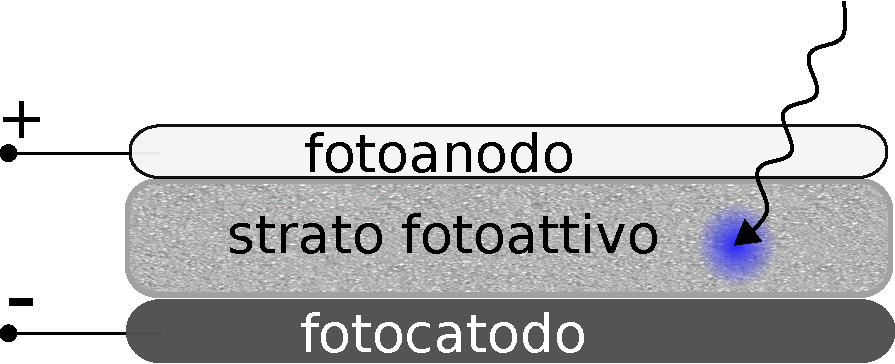
\includegraphics[width=.55\textwidth]{Immagini_Tesi/pv-schema1.pdf}}
\caption{\footnotesize{Uno schema generale di cella fotovoltaica.}
\label{fig:pv-schema1}}
\end{figure}

\section{Fotovoltaico}
Una cella fotovoltaica è un dispositivo atto a convertire energia luminosa in energia elettrica. Lo schema generale di una cella fotovoltaica è riportato in~\ref{fig:pv-schema1}.
Le funzioni, illustrate in~\ref{fig:livelli}, che devono essere svolte dai componenti di una cella sono:
\begin{enumerate}[label=\roman{*}.]
\item assorbimento della luce e fotogenerazione delle cariche,
\item trasporto delle cariche fino agli elettrodi,
\item trasferimento delle cariche sugli elettrodi.
\end{enumerate}

\begin{figure}
\centering{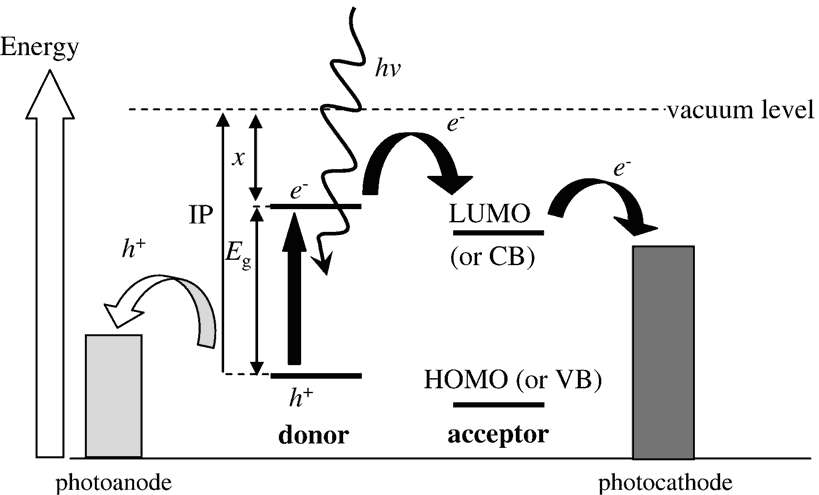
\includegraphics[width=.8\textwidth]{Immagini_Tesi/livelli.png}}
\caption{\footnotesize{Schema dei livelli energetici e della storia di una fotoeccitazione. Immagine tratta da \cite{fv-all}.}
\label{fig:livelli}}
\end{figure}
Le celle fotovoltaiche attualmente più diffuse sono basate sul silicio. 
Purtroppo è necessario utilizzare silicio ad elevati gradi di purezza (comunque inferiori al silicio per applicazioni elettroniche) e questo causa l'alto costo dei pannelli fotovoltaici classici.  
       
Per ovviare al problema del costo sono state sviluppate nuove combinazioni di materiali per applicazioni fotovoltaiche. 
Negli ultimi anni sono stati sviluppati materiali fotoattivi composti da nanoparticelle e polimeri semiconduttori. Le nanoparticelle utilizzate possono essere organiche o inorganiche ma in ogni caso si tratta di semiconduttori. Per i semiconduttori inorganici in forma di nanoparticelle si adotta il nome di \emph{quantum dots}\footnote{Quantum dot: materiale in cui i portatori di carica hanno zero gradi di libertà spaziale. Definizione data ma Mark Reed nel 1986.}. Inoltre queste nanoparticelle possono essere sferiche, a bacchetta o ramificate ( vedi~\ref{fig:NPs}).
          
I polimeri semiconduttori sono polimeri con una estesa coniugazione di doppi legami.        

Nei semiconduttori, a causa della loro struttura a bande illustrata in~\ref{fig:semicond-schema1}, non si ha presenza di cariche e lacune libere di condurre se il materiale si trova nello stato fondamentale. Una radiazione elettromagnetica con energia maggiore del \emph{band gap} può generare stati eccitati in cui si hanno elettroni nella banda di conduzione e lacune nella banda di valenza. Collegando questo semiconduttore con degli elettrodi metallici con livelli di Fermi\footnoteremember{Fermi}{{\descriptionlabel{Livello di Fermi}} allo zero assoluto coincide con l'energia di Fermi, ossia lo stato quantistico a più alta energia che risulta popolato allo zero assoluto. Invece a temperature maggiori è il potenziale chimico degli elettroni che compare nella distribuzione di Fermi-Dirac.} ad energia opportuna è possibile accumulare queste cariche ed ottenere una differenza di potenziale.
\begin{figure}
\centering{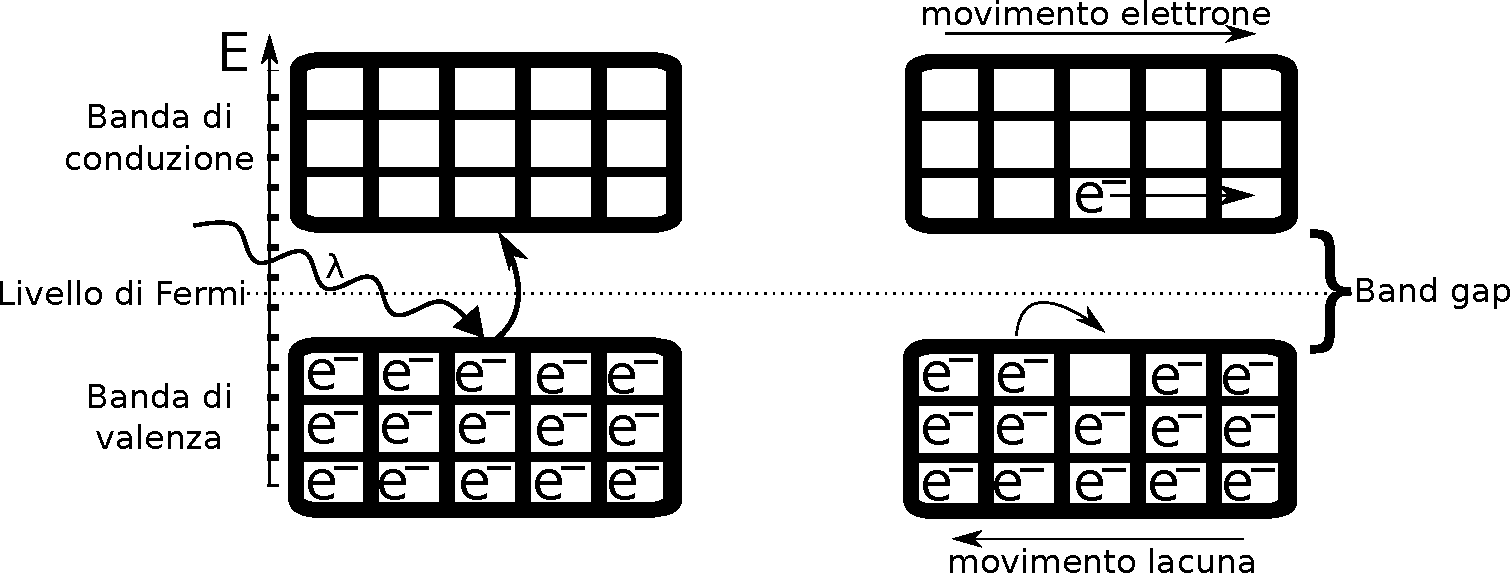
\includegraphics[width=.8\textwidth]{Immagini_Tesi/semicond-schema1.pdf}}
\caption{\footnotesize{Uno schema generale di sermiconduttore.}
\label{fig:semicond-schema1}}
\end{figure}

\subsection{Fotogenerazione di eccitoni}
Le radiazioni dello spettro solare possono venir assorbite da uno o da entrambi i semiconduttori presenti nello strato fotoattivo in funzione del loro \emph{band gap} (un materiale con \emph{band gap} minore assorbe una maggiore porzione dello spettro). Inoltre è possibile utilizzare un ``colorante'' inserito nello strato appositamente per fotogenerare cariche. Nel caso in studio sia le nanoparticelle che il polimero assorbono nel visibile e non verranno aggiunti coloranti. 
        

I polimeri coniugati hanno tipicamente una differenza LUMO - HOMO maggiore di 2~eV, corrispondente all'energia di un fotone con $\lambda=600$~nm. Con un tale \emph{band gap} i polimeri sono in grado di assorbire solo il 30\% della radiazione solare \cite{fv-eccit}. 
        

I fotoni assorbiti possono dare fotoeccitazioni diverse in dipendenza dalla loro energia che può essere maggiore o minore del \emph{band gap}. Nel primo caso l'energia è sufficiente a generare una lacuna ed un elettrone liberi ma le misurazioni danno per questo evento una resa quantica solamente di $\phi_{ch}\approx10\%$ \cite{pol-polarons}. Il restante 90\% e le radiazioni meno energetiche generano uno stato eccitato della materia detto eccitone. Questo è costituito da un elettrone e da una lacuna legati ossia che non hanno ricevuto energia sufficiente per separarsi. Recuperare l'energia contenuta negli eccitoni permetterebbe di aumentare molto l'efficienza energetica\footnoteremember{PCE}{{\descriptionlabel{Efficienza energetica (Power Conversion Efficiency PCE)}} rapporto tra la massima potenza in uscita e la potenza incidente in ingresso.} della cella fotovoltaica.
\subsection{Separazione delle cariche}
La separazione delle cariche che legate costituiscono l'eccitone è possibile se questo incontra una zona di forte campo elettrico \cite{fv-pcbm}. Questo si può generare all'interfaccia tra due materiali in cui si ha un accumulo di cariche. Questo accumulo si forma spontaneamente per mantenere l'uniformità spaziale del livello di Fermi \footnoterecall{Fermi} e per congiungere le bande di valenza e conduzione.
Il raggiungimento di questo equilibrio è illustrato in~\ref{fig:depletion_layer}.
\begin{figure}
\centering{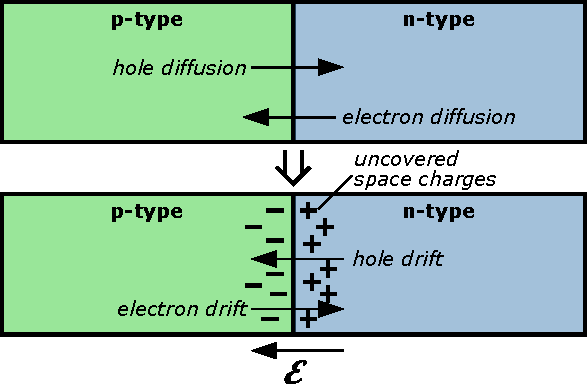
\includegraphics[width=.6\textwidth]{Immagini_Tesi/depletion_layer.pdf}}
\caption{\footnotesize{Sopra: giunzione $p-n$ prima della diffusione; sotto: dopo il raggiungimento dell'equilibrio. Immagine tratta da Wikimedia.}
\label{fig:depletion_layer}}
\end{figure}
\subsection{Trasporto delle cariche}
\label{sec:trasporto}
Una volta separate, le cariche devono essere trasportate fino agli elettrodi. Il movimento è indotto dal potenziale dei materiali utilizzati negli elettrodi come schematizzato in~\ref{fig:livelli}. Per limitare la ricombinazione tra cariche negative e lacune positive si utilizzano due materiali diversi per il trasporto. Questi possono essere gli stessi che costituiscono l'interfaccia, nel caso in studio il polimero semiconduttore e le nanoparticelle semiconduttrici. Per ottenere una buona conduzione si vuole una continuità all'interno di ciascun semiconduttore, ossia deve esistere un percorso di semiconduttore che connetta l'interfaccia interna al bordo dello strato fotoattivo. Nel caso della fase polimerica si deve considerare che le cariche non sono libere quanto in un semiconduttore inorganico, bensì deve aver luogo anche un trasporto intercatena. Questo trasporto viene reso più difficoltoso dalla presenza delle catene laterali alifatiche tipicamente presenti sul polimero e necessarie per rendere solubile il polimero stesso.
\subsection{Morfologia}
Un eccitone si propaga per brevi distanze, tipicamente 10nm in un semiconduttore organico \cite{fv-CdSe-OA}, prima di decadere radiativamente. Per avere una separazione efficace delle cariche è necessario che gli eccitoni incontrino una interfaccia nel loro breve tempo di vita. Le prime celle a polimeri erano costituite di due strati di polimero sovrapposti (morfologia \emph{bilayer}): uno per il trasporto degli elettroni ed uno per il trasporto delle lacune (vedi~\ref{fig:bilayer-bulk-heterojunction}).

\begin{figure}[!htb]
\centering{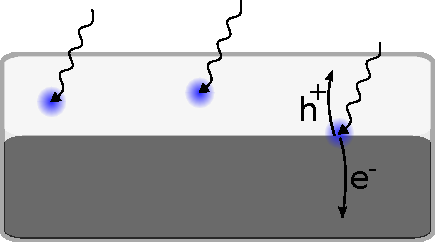
\includegraphics[width=.385\textwidth]{Immagini_Tesi/bilayer-eccitoni.pdf}
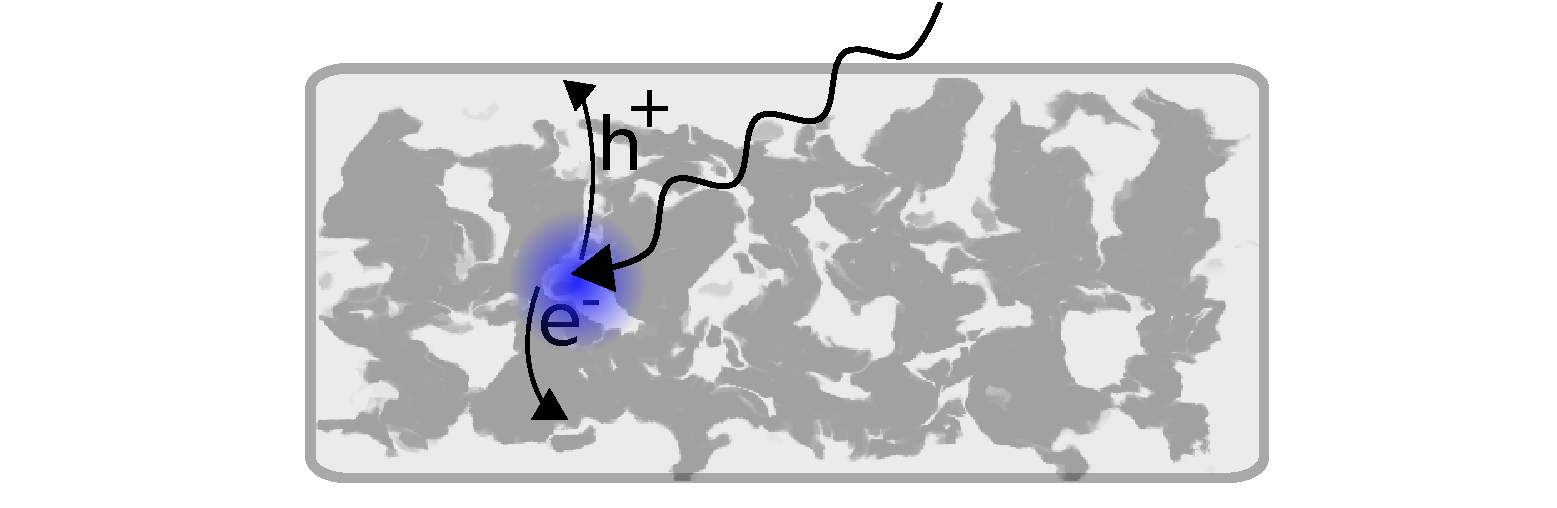
\includegraphics[width=.605\textwidth]{Immagini_Tesi/bulk-heterojunction-eccitoni.pdf}\\
\makebox{\parbox[b]{.385\textwidth}{\centering{(a)}}}
\makebox{\parbox[b]{.605\textwidth}{\centering{(b)}}}}
\caption{\footnotesize{Alcune morfologie: (a) \emph{bilayer}, (b) \emph{bulk heterojunction}. }}
\label{fig:bilayer-bulk-heterojunction}
\end{figure}
  

In queste celle la maggior parte degli eccitoni decadeva radiativamente prima di raggiungere l'interfaccia e di essere spezzati in cariche. Perciò una morfologia che può dare efficienze energetiche\footnoterecall{PCE} maggiori ha una interfaccia distribuita nello strato attivo: un \emph{bulk heterojunction}. Il \emph{bulk heterojunction} è illustrato in~\ref{fig:bilayer-bulk-heterojunction}-(b).
Il problema principale di una morfologia \emph{bulk heterojunction} si incontra nella sua formazione: i due semiconduttori non sono miscibili tra loro e tendono a separarsi dando estese aggregazioni come illustrato in~\ref{fig:interconnessi-allineati}-(a). Confrontandole con le nanoparticelle organiche, le inorganiche hanno una tendenza ad aggregarsi molto maggiore.
\setlength{\captionmargin}{.05\textwidth}  
\begin{figure}[!htb]
\centering{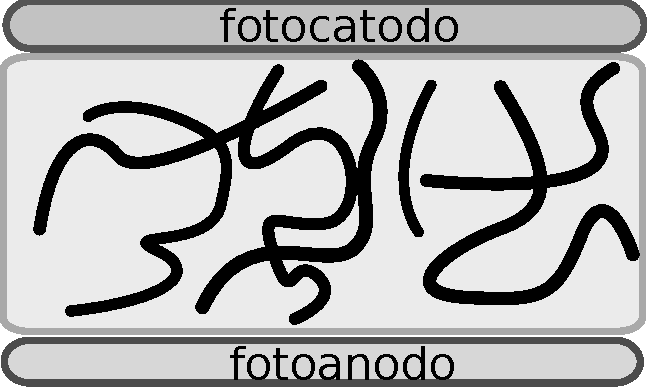
\includegraphics[width=.476\textwidth]{Immagini_Tesi/interconnessi_poco_aggregati.pdf}
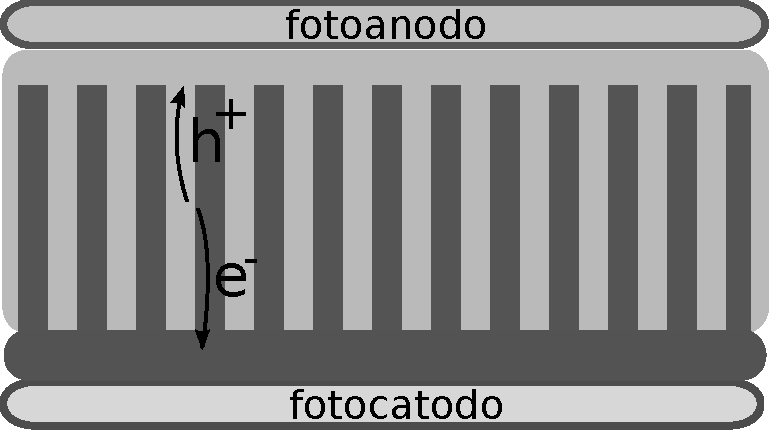
\includegraphics[width=.514\textwidth]{Immagini_Tesi/aggregati_allineati.pdf}\\
\makebox{\parbox[b]{.476\textwidth}{\centering{(a)}}}
\makebox{\parbox[b]{.514\textwidth}{\centering{(b)}}}}
\caption{\footnotesize{(a) La tendenza ad aggregarsi delle nanoparticelle produce sistemi con minore superficie di interfaccia. \\(b) La morfologia ideale per una cella solare \emph{bulk heterojunction}. }}
\label{fig:interconnessi-allineati}
\end{figure}
\setlength{\captionmargin}{.10\textwidth} 

Un possibile approccio volto ad aumentarne la miscibilità o comunque la dispersibilità in una matrice costituita dal polimero coniugato consiste nella modifica di una porzione del polimero coniugato introducendo funzionalità leganti nei confronti delle nanoparticelle. Questo verrà discusso nella Sottosezione~\ref{subsec:polimeri_cond}.

La morfologia ideale delle due fasi è costituita dalle fasi allineate verticalmente \cite{fv-morf-allineata} come illustrato in~\ref{fig:interconnessi-allineati}-(b). In questa struttura si minimizzano le ricombinazioni. La percolazione delle due fasi termina prima degli elettrodi per impedire la collezione di cariche di segno sbagliato sugli stessi.
      

Il problema principale consiste, come facilmente intuibile, nella difficoltà di ottenere tale morfologia con processi di fabbricazione o di autoassemblaggio.

\section{Caratteristiche dei materiali}

\subsection{Nanoparticelle}
\begin{figure}
\centering{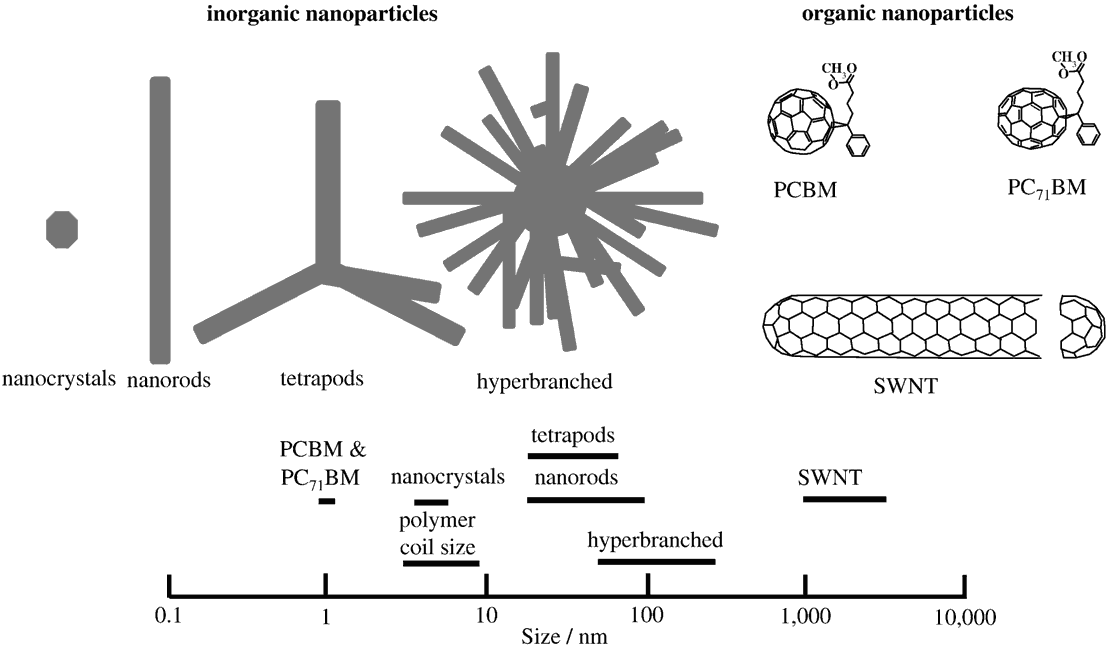
\includegraphics[width=.7\textwidth]{Immagini_Tesi/NPs2.png}}
\caption{\footnotesize{Esempi di nanoparticelle: a sinistra inorganiche, a destra organiche. Immagine tratta da \cite{fv-all}.}
\label{fig:NPs}}
\end{figure}
Le nanoparticelle possono essere semiconduttori organici o inorganici. In entrambi i casi vengono utilizzate come accettori e trasportatori di elettroni. Sia le organiche che le inorganiche possono avere forma sferica o più complessa ( vedi~\ref{fig:NPs} ). In questo lavoro verranno sintetizzate solo nanoparticelle inorganiche (nanocristalli) le quali presentano i seguenti vantaggi e svantaggi:
\begin{itemize}
 \item[\checkmark] i livelli energetici possono esser variati con la dimensione,
 \item[\checkmark] hanno alti coefficienti di assorbimento della luce,
 \item[\checkmark] hanno una mobilità elettronica più alta delle nanoparticelle organiche \cite{fv-CdSe-OA},
 \item[$\times$] le efficienze ottenibili sono in genere più basse a causa della maggiore aggregazione \cite{fv-all}, 
 \item[$\times$] l'uso dei metalli pesanti utilizzati è limitato per via della loro tossicità,
 \item[$\times$] hanno dimensioni maggiori delle nanoparticelle sferiche organiche (PCBM) perciò risulta una minore superficie interfacciale \cite{fv-all}.
\end{itemize}
La forma delle nanoparticelle sarà sferica per semplicità di sintesi. 
In letteratura si trovano molti materiali semiconduttori utilizzabili per i nostri scopi: TiO$_2$, ZnO, PbS, CdSe, CdTe, CuInSe$_2$, CuInS$_2$, CdS, PbSe, GaAs \ldots In questo lavoro si utilizzeranno nanocristalli sferici di CdSe. Per questo semiconduttore la letteratura riporta le efficienze energetiche più alte \cite{fv-all}. Inoltre è possibile la sintesi di nanofili e di strutture ramificate di CdSe per ulteriori sviluppi di questi sistemi verso efficienze più elevate. 
\subsection{Polimeri semiconduttori}

\label{subsec:polimeri_cond}
I polimeri semiconduttori sono molecole con una estesa coniugazione di doppi legami e/o sistemi aromatici. Hanno la funzione sia di assorbire la luce sia di donare elettroni e di trasportare lacune. 
        
I polimeri semiconduttori più usati per applicazioni nel fotovoltaico organico o ibrido sono idrofobici e sono elencati in~\ref{fig:polimericonduttori}.
\setlength{\captionmargin}{-.05\textwidth}
\begin{figure}
\centering{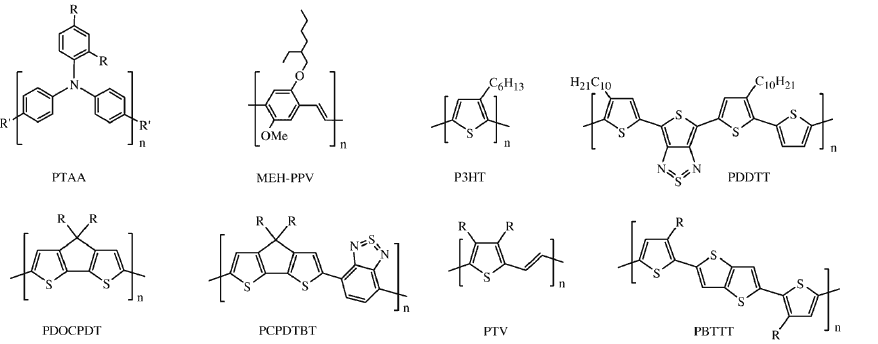
\includegraphics[width=.9\textwidth]{Immagini_Tesi/polimericonduttori2.png}}
\caption{\footnotesize{Struttura dei polimeri semiconduttori utilizzati nelle celle fotovoltaiche. PTAA: poli(triarilammina); MEH-PPV: poli(2-metossi-5-etilesilossifenilene vinilene); P3HT: poli(3-esiltiofene); PDDTT: poly[5,7-bis(4-decanyl-2-thienyl)thieno[3,4-b]diathiazole-thiophene-2,5)]; PDOCPDT: poly[2,5-(7,7-dioctyl)-cyclopentadithiophene]; PCPDTBT: poly[2,6-(4,4-bis-(2-ethyhexyl)-4H-cyclopenta[2,1-b;3,4-b′]-dithiophene)-alt-4,7-(2,1,3-benzothiadiazole)]; PTV: poli(tienilene vinilene); PBTTT: poly[2,5-bis(3-alkylthiophen-2-yl)thieno[3,2-b]thiophene)].
Immagine tratta da \cite{fv-all}}
\label{fig:polimericonduttori}}
\end{figure}
        
In un polimero coniugato il \emph{band gap} è la differenza LUMO - HOMO\@. Questi corrispondono rispettivamente alla banda di conduzione e di valenza. 

Solitamente la separazione è maggiore di 2~eV, perciò l'energia termica a temperatura ambiente non è sufficiente a popolare il LUMO ed il polimero risulta un semiconduttore.
Se a questo viene donato o sottratto un elettrone allora diventerà conduttore (vedi~\ref{fig:semicond-schema1}). Ciò avviene durante la separazione degli eccitoni formati con l'assorbimento dei fotoni. 
\setlength{\captionmargin}{.0\textwidth}  

\begin{wrapfigure}{r}{0.50\textwidth}
\begin{center}
    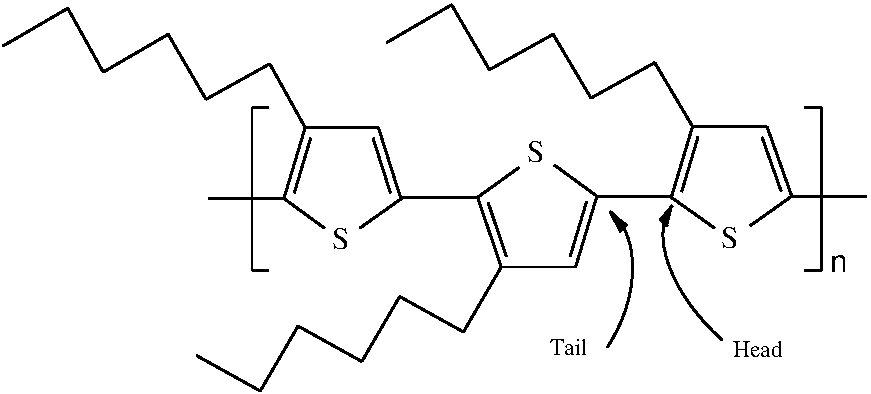
\includegraphics[width=1\textwidth]{Immagini_Tesi/p3ht-htht.pdf}
  \end{center}
  \vspace{-5pt}\footnotesize{\caption{Poli(3-esiltiofene) regioregolare \emph{head-tail-head-tail}.\label{fig:p3ht-htht}}}
\end{wrapfigure}
\setlength{\captionmargin}{.10\textwidth}  
      
La differenza LUMO - HOMO dipende dal monomero e diminuisce con la lunghezza di coniugazione fino al raggiungimento di 15-20 unità monomeriche, oltre la quale si stabilizza. Perché questa coniugazione sia presente è necessario che il polimero sia planare. 


La sua planarità (ed il trasporto intercatena, vedi Sottosezione~\ref{sec:trasporto}) è disturbata dalla repulsione tra le catene laterali alifatiche necessarie per rendere il polimero solubile in solventi organici e quindi lavorabile, tipicamente per deposizione su un supporto tramite \emph{spin coating}. 


Questa interazione può essere minimizzata nel caso di polimeri con unità ripetenti a struttura asimmetrica sintetizzando un polimero regioregolare \emph{head-tail-head-tail}\label{regio-htht}, vedi~\ref{fig:p3ht-htht}. 
 
Il polimero che verrà sintetizzato in questa tesi è il poli(3-esiltiofene). Questa scelta è motivata dal fatto che i livelli energetici del CdSe sono adatti ad essere accoppiati con quelli del politiofene: la differenza energetica tra il LUMO del polimero donatore e la banda di conduzione delle nanoparticelle accettrici (vedi~\ref{fig:livelli}) deve essere non troppo piccola ma nemmeno troppo grande per evitare la popolazione di stati di tripletto del polimero. Inoltre è stato riportato in letteratura che la lunghezza massima di coniugazione raggiunge le 20 unità monomeriche \cite{pol-pti-lunghezza}. 

